% Faz com que o inicio do capítulo sempre seja uma página ímpar
\cleardoublepage
% Inclui o cabeçalho definido no meta tex
\pagestyle{fancy}
% Números das páginas em arábicos
\pagenumbering{arabic}

\chapter{Introdução}\label{intro}

\section{Modularidade}\label{intro:modularidade}

Na imensa maioria dos organismos, conseguimos identificar partes relativamente discretas
e separadas, frequentemente envolvidas no desempenho de alguma função.
Em organismos unicelulares podemos distinguir organelas desempenhando
funções específicas, bem como regiões internas ou na membrana responsáveis por
processos distintos.
Já nos multicelulares, tipos celulares são organizados em tecidos espacialmente
separados, formando órgãos de funções distintas, que por sua vez são
organizados em sistemas responsáveis por funções distintas.
Modularidade se refere a esse padrão de organização dos seres vivos, onde
algumas partes são mais relacionadas entre si do que com outras partes
do mesmo organismo.
Podemos descrever, e entender, a organização entre partes
constituintes dos organismos através das relações entre elas, sendo cada
tipo de relação adequada a um nível de complexidade ou organização.
As partes do organismo as quais nos referimos podem ser as bases
nitrogenadas de uma molécula de RNA \citep{Ancel2000}, genes
\citep{Costanzo2010}, proteínas \citep{Han2004}, caracteres morfológicos
como peso, altura ou marcos anatômicos \citep{Klingenberg2008,
Porto2009, Marroig2009}.
Essas relações podem ser medidas de diversas formas, como interação física
entre proteínas, padrões de expressão conjunta entre genes, ou, como é o caso
no presente trabalho, correlação entre caracteres quantitativos.
Esse grupo de características muito relacionadas entre si constituem um
módulo, como esquematizado na figura \ref{modulos}.
Módulos, então, são caracterizados por uma alta conectividade interna e
relativa independência de outros módulos.

A formação desses módulos reflete uma complexa interação entre genes,
desenvolvimento e ambiente, e tem consequências diversas para o
funcionamento e evolução dos seres vivos \citep{Wagner1996}.
Talvez o aspecto funcional seja o ponto de partida mais simples para
entender a origem da organização modular.
Interação com o ambiente e a necessidade de realizar determinada função
provoca respostas evolutivas nas populações, privilegiando o surgimento
de estruturas e sistemas adaptados para realizar essas funções.
Para que essas estruturas possam se adequar às diferentes pressões
evolutivas que cada parte do organismo está sujeita, uma relativa
independência entre elas se estabelece \citep{Wagner2007, Klingenberg2008}.
Essa independência se estabelece em vários níveis.
Através de experimentos controlados de cruzamento e uso de marcadores
genéticos, é possível mapear regiões no genoma envolvidas com
determinação de características macroscópicas nos organismos.
Com essas metodologias foi verificado que loci tendem a influenciar
regiões discretas, sendo poucos os genes com efeitos entre regiões
funcionais diferentes \citep{Cheverud1997}.
Genes que influenciam mais de uma característica de um indivíduo são
denominados pleiotrópicos.
Ou seja, seleção privilegia pleiotropia restrita a regiões funcionais
distintas \citep{Cheverud1984}.
Além disso, as estruturas e processos ontogenéticos responsáveis pela
formação dos indivíduos apresentam uma independência relativa, sendo
possível alterar parte do processo ou estrutura sem um efeito cascata
sobre outros processos ou estruturas \citep{Klingenberg2008}
Talvez o exemplo mais simples seja imaginar um organismo onde todos os
caracteres ou processos ontogenéticos estejam integrados (altamente
correlacionados) entre si, ou, dito de outra forma, pertencentes ao mesmo módulo.
Nesse organismo qualquer mudança em qualquer caráter ou processo levaria
a alterações em todos os outros.
Uma alteração pode ser benéfica em um caráter, mas deletéria em vários
outros.
A modularidade evita essa cenário, permitindo com que partes
independentes se alterem de forma relativamente independente.
O outro lado da moeda são os processos de integração, resultantes da
necessidade do organismo de manter a coerência interna dos seus módulos
e do indivíduo como um todo.
Integração leva a aumento da coesão entre as características
do organismo.
Evolutivamente, integração e modularidade permitem que grupos de
características funcionalmente ou ontogeneticamente ligadas se
modifiquem de forma harmoniosa; e que características em módulos
diferentes possam se alterar de forma relativamente independente
.

\begin{figure}[h!]
  \centering
  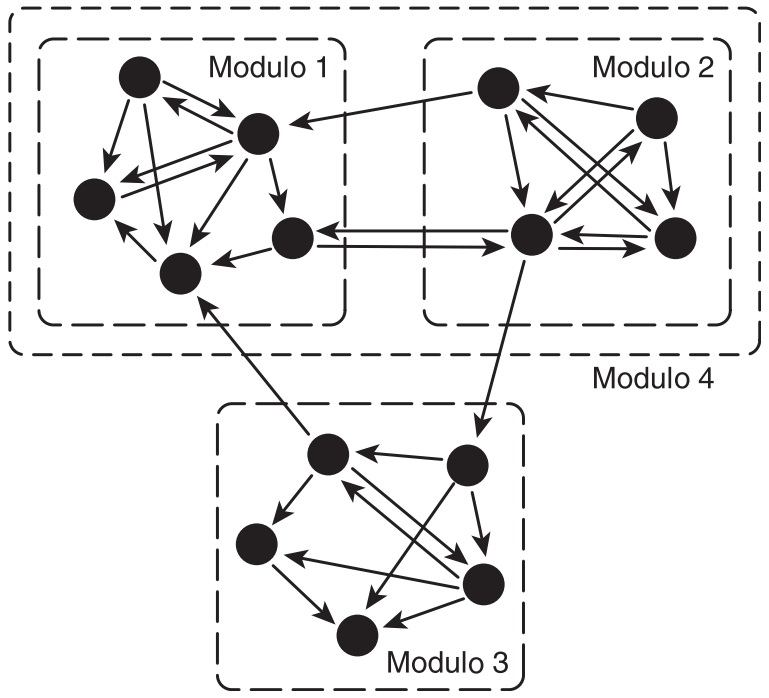
\includegraphics[width=100mm]{figuras/modulos.png}
  \caption{Representação esquemática da organização modular dos seres
  vivos.
  As setes representam qualquer tipo de relação entre as partes
  de um indivíduo.
  Adaptado de \cite{Klingenberg2008}}
  \label{modulos}
\end{figure}

Em caracteres quantitativos, descritos em detalhe na seção
\ref{intro:genquant}, a expressão de todos os processos genéticos,
ontogenéticos e ambientais que formam a organização modular do organismo se
dá na forma de covariação (ou correlação) entre os caracteres.
Ou seja, o conflito entre os processos de modularidade e integração em todos os
níveis de organização do indivíduo podem ser percebidos na estrutura de
covariação final da população \citep{Klingenberg2008}.
Módulos caracterizados por alta correlação entre caracteres dentro do
módulo e baixa correlação entre caracteres de módulos diferentes são
chamados de módulos variacionais \citep{Wagner2007}.
Estes são frequentemente identificados como relacionados a funções
específicas, como mastigação, inserção muscular ou proteção
\citep{Cheverud1997}.
Novamente, seleção privilegia interações pleiotrópicas e ontogenéticas restritas
a características ligadas a uma função comum, que resulta em
covariação entre essas características na população.


\section{Genética Quantitativa e Modularidade}\label{intro:genquant}

O estudo de caracteres quantitativos se baseia amplamente na teoria da
genética quantitativa.
A genética quantitativa estuda a herança de características contínuas
nos indivíduos de uma população, como peso, altura ou taxas de
crescimento \citep{Falconer1996}.
A partir desse formalismo, originário do melhoramento genético de animais e plantas, 
podemos prever como a média e distribuição de
características fenotípicas varia em uma população de uma geração para
outra.

Caracteres contínuos são usualmente determinados geneticamente por muitos loci,
sendo portanto denominados caracteres poligênicos.
A influência exata de cada um desses loci no fenótipo do individuo é
desconhecida, porém a combinação de todos esses efeitos e dos efeitos
ontogenéticos e ambientais resultam no valor fenotípico observado.
Em \cite{Crow1964} e \cite{Kimura1965} os autores descrevem um modelo
para os efeitos alélicos agindo sobre caracteres contínuos.
Neste modelo, chamado modelo do continuo de alelos, cada locus em
principio pode ter qualquer efeito sobre o tamanho de um caráter,
aumentando ou diminuindo seu valor fenotípico, e
qualquer um desses efeitos pode ser atingido via mutação.
A enorme variabilidade possível em sequências genéticas e o número de
loci controlando cada caráter garante que essa suposição seja verossímil.
Nesse contexto, o valor fenotípico de um caráter $p$ é dado pela soma dos
efeitos genéticos ($g$) e ambientais ($e$) atuando sobre ele:

\begin{equation}
    p = g + e
\end{equation}

A variação total de uma dada característica é resumida na sua variância
fenotípica, denominada $V_p$.
Esse valor de variância total é fruto da variação genética ($V_g$)
presente na população e da variação devido ao ambiente no qual a
população se encontra ($V_e$), além da possível interação entre elas.
Como as variâncias são aditivas, podemos escrever:

\begin{equation}
    V_p = V_g + V_e + V_{g \cdot e}
\end{equation}

Em organismos com sistemas de desenvolvimento estáveis, relativamente tamponados,
como é o caso dos mamíferos, podemos em geral ignorar o termo de interação em
genótipo e ambiente ($V_{g \cdot e} = 0$).
Podemos continuar particionando as variâncias.
A variância genética é resultado de toda a variação devido ao efeito
aditivo dos alelos ($V_a$, variância aditiva), mais os efeitos não
aditivos, efeitos de dominância ($V_d$, não aditivos) e efeitos
epistáticos ($V_{i}$, representando interações entre diferentes loci).
Ou seja:

\begin{equation}
    V_g = V_a + V_d + V_{i}
    \label{compgen}
\end{equation}

O termo aditivo, $V_a$, representa a porção da variância genética
responsável pela semelhança por parentesco.
Isso se reflete na equação de resposta à seleção direcional univariada.
A pressão seletiva sobre alguma característica fenotípica pode ser descrita
pela diferença na média da população parental antes ($\overline p$) e depois
($\overline p^*$) do evento de seleção.
Essa quantidade é denominada diferencial de seleção e é representada por
$S$.
Esse tipo de seleção, que afeta média de um caráter na população, é
chamado de seleção direcional.
A resposta observada na média na geração seguinte ($\Delta \overline z$) é dada
por:

\begin{equation}
    \Delta z = \frac{V_a}{V_p} (\overline p^* - \overline p) = h^2S
\end{equation}

Ou seja, a parcela da variância fenotípica devido à variação genética
aditiva define o quão eficiente será a resposta da população à seleção
direcional.
Essa parcela é denominada herdabilidade, representada por $h^2$.
Mas essa equação ignora o efeito de seleção indireta em outras
características do indivíduo.
Para levar em conta esses efeitos, devemos
lançar mão de um formalismo multivariado.

A equação multivariada de resposta à seleção,
proposta por \cite{Lande1979}, permite ligar a mudança na média de um
conjunto de caracteres ($\Delta \mathbf{z}$) ao diferencial de seleção imposto à população
($\mathbf{S}$) e à suas matrizes de covariação genética aditiva e fenotípica
($\mathbf{G}$ e $\mathbf{P}$).

\begin{equation}
    \Delta \mathbf{z} = \mathbf{GP}^{-1}\mathbf{S}
    \label{landeZGS}
\end{equation}
 
$\Delta \mathbf{z}$ e $\mathbf{S}$ agora são vetores de mesma dimensão que o número
de características consideradas na analise.
As variâncias são expressas nas matrizes $\mathbf{G}$ e $\mathbf{P}$, que são os análogos
multivariados das quantidades $V_a$ e $V_p$.
O caso multivariado apresenta um comportamento qualitativamente
diferente do caso univariado.
Como os caracteres são ligados por efeitos genéticos correlacionados,
representados pela matriz $\mathbf{G}$, a seleção direcional não é capaz de atuar de
forma isolada em cada caráter.
Seleção direcional, ainda que restrita a um caráter, provoca respostas
evolutivas em todos os caracteres que covariam com o caráter sobre
seleção.

Utilizando o conceito de superfície de seleção, proposto por
\cite{Wright1932}, podemos interpretar o termo de seleção
$\mathbf{P}^{-1}\mathbf{S}$ de forma geométrica.
A superfície de seleção associa cada valor fenotípico para todos os
caracteres a um valor de aptidão ou {\it fitness}.
Caso essa superfície seja gaussiana, \cite{Lande1983} mostraram que
$\mathbf{P}^{-1}\mathbf{S}$ é equivalente ao gradiente da média da
superfície de seleção na população.
O gradiente de um campo escalar, como é caso da superfície de seleção,
é definido como o campo vetorial que aponta para a direção de maior
variação do campo escalar, com magnitude igual a taxa de variação do
campo escalar.
Ou seja, o gradiente em cada ponto da superfície de seleção indica qual
é a direção de mudança fenotípica que mais aumenta a aptidão da
população que se encontra nesse ponto do morfoespaço.
Por esse motivo, a quantidade $\mathbf{P}^{-1}\mathbf{S}$ é chamada
de gradiente de seleção, e é representada pelo vetor $\beta$.
Nas próximas seções vamos nos referir também a seleção estabilizadora.
Esse tipo de seleção age sobre a distribuição de um caráter, diminuindo
sua variabilidade, mas não sobre a média do caráter.
Com respeito à superfície de seleção, a seleção estabilizadora é
resultado da curvatura da superfície, ou da sua Hessiana
\citep{Lande1983}.
No caso de seleção direcional, podemos escrever a equação de resposta a
seleção como:

\begin{equation}
    \Delta z = \mathbf{GP}^{-1}S = \mathbf{G}\beta
    \label{landeZGBETA}
\end{equation}

A evolução dos caracteres por seleção direcional toma a forma de uma
subida de gradiente da superfície de seleção, alterado pela estrutura de
covariação genética, representada pela matriz $\mathbf{G}$.

\section{Evolução da matriz $\mathbf{G}$ e a resposta à seleção}\label{intro:matG}

Na seção \ref{intro:modularidade}, nós descrevemos como os processos
seletivos interagem com o desenvolvimento e arquitetura genética das
populações ,gerando modularidade.
Dissemos também que a modularidade presente nos processos internos dos
organismos se manifesta na população na sua estrutura de covariação.
Essa estrutura de covariação é representada pela matriz $\mathbf{G}$.
Ela descreve como a variação aditiva, herdável, da população está particionada entre os
seus caracteres, e como estes se relacionam entre si.
Caracteres associados por efeitos pleiotrópicos e ontogenéticos irão
apresentar covariação alta, enquanto caracteres independentes, não
relacionados, irão apresentar covariação baixa.
Como a população responde à seleção direcional, portanto, depende da sua estrutura
de modularidade e de como os caracteres estão relacionados entre si.

A equação de \cite{Lande1979} também pode ser invertida e usada de forma
retrospectiva.
Ou seja, partindo da matriz $\mathbf{G}$ e da diferença observada entre as médias
antes de depois do evento de seleção, podemos inferir qual foi o
gradiente de seleção que gerou essa resposta.
Mais claramente:

\begin{equation}
    \beta = \mathbf{G}^{-1}\Delta \mathbf{z}
\end{equation}

Além disso, esse mesmo raciocínio pode ser usado para investigar padrões
macroevolutivos de resposta ao longo de muitas gerações
\citep[veja também a equação \ref{betatotal}]{Lande1983, Marroig2004, Marroig2005}.

Porém, nossa habilidade de inferir a resposta evolutiva a muitas
gerações de seleção depende fundamentalmente da constância da matriz G
ao longo do tempo, e a teoria de Lande não explora
detalhadamente a dinâmica da própria matriz $\mathbf{G}$, assumindo implicitamente
nas equações sua constância.
Dizer que a distribuição das características na população é 
gaussiana implica que essa distribuição não é afetada pela seleção direcional
\citep{Barton1987}.
Isso se reflete na equação de resposta a seleção direcional, que envolve
apenas mudanças na média dos caracteres.
Essa suposição simplificadora de Lande se baseia em um resultado
derivado do modelo do continuo de alelos, demonstrado por
\cite{Kimura1965}: sobre seleção estabilizadora, a
distribuição de equilíbrio dos efeitos alélicos sobre um determinado
caráter é gaussiana, supondo que os efeitos mutacionais sejam pequenos
frente à variação existente na população.
Ou seja, assumindo que os efeitos alélicos sejam efetivamente
gaussianos, a dinâmica da média da população pode ser completamente
descrita apenas pela média e pela matriz de covariação desses efeitos
\citep{Barton1987}.

Notamos então que uma série de suposições não triviais devem ser feitas
para que esse modelo gaussiano quadrático de Lande seja teoricamente
plausível.
Esses problemas foram apresentados ao longo da década de 80 por uma
série de artigos, principalmente e pioneiramente por \cite{Turelli1984,
Turelli1985, Turelli1986, Barton1987, Barton1989}.
Talvez a questão mais importante seja a suposição de que os alelos
tenham distribuição gaussiana proposta por \cite{Kimura1965}.
Para que isso seja realista, a taxa de mutação por locus deve ser
suficientemente alta para manter a distribuição de alelos por locus
gaussiana frente à deriva e seleção estabilizadora, que removem
variabilidade \citep{Falconer1996}.
Além disso, podemos nos perguntar se mutações novas realmente tem efeitos
pequenos em relação a variância original da população nas direções
morfológicas afetadas, ou se novas mutações introduzem variabilidade
maior que a originalmente presente na população.
O modelo proposto por \cite{Turelli1984} utiliza taxas de mutação
baixas e efeitos mutacionais altos, mas ainda mantendo o espaço de
alelos contínuo.
Neste modelo, a maior parte da variação fenotípica acaba sendo atribuída
a alelos raros, de baixa frequência, mas com efeitos aditivos grandes, e
não a vários alelos polimórficos de efeitos pequenos e distribuição
gaussiana.
Nessas condições, a matriz $\mathbf{G}$ não seria constante ao longo do tempo e
fatores de correção deveriam ser acrescidos à equação de resposta de
Lande para descrições macro evolutivas.
Esses fatores dependem do desvio por geração da matriz $\mathbf{G}$ em relação à
matriz $\mathbf{G}$ média no período de seleção \citep{Jones2004}.
A estimativa desse ``efeito Turelli'' é difícil de ser realizada
praticamente.

Em \cite{Barton1987}, os autores, interessados no problema da dinâmica
das variâncias de forma geral, apresentam um formalismo relativamente
completo para lidar com o problema da evolução de todos os momentos da
distribuição fenotípica de um caráter quantitativo, abordando tanto a
aproximação gaussiana quanto a aproximação de alelos raros, proposta por
\cite{Turelli1984}.
O procedimento seguido pelos autores é escrever a dinâmica de mudança de
todos o momentos da distribuição de efeitos alélicos da população
sujeita a uma pressão de seleção na forma de uma subida de gradiente
imposta por uma superfície de seleção arbitrária (mas com todas as
derivadas parciais bem definidas no espaço dos momentos)
\citep{Arnold2001a}.
Isso permite abarcar o formalismo de Lande, tomando apenas os dois
primeiros momentos (média e variância), supondo o segundo momento fixo e
desprezando os momentos mais altos; ou incluir mudanças até uma certa
ordem e obter os resultados de Turelli.
Por outro lado, a descrição do sistema baseada nos seus momentos é
analiticamente bastante complicada, e não permite a inclusão de
epistasia (interação entre loci) de forma simples.
Posteriormente, buscando um formalismo mais natural e genérico para a
evolução de caracteres quantitativos associados por correlações
genéticas, os mesmo autores em \cite{Turelli1994} apresentam um
formalismo baseado nos cumulantes da distribuição de efeitos alélicos.
Apesar de menos intuitivo, o formalismo baseado em cumulantes é mais
simples no caso de alelos aditivos, e fornece equações
recursivas para a evolução dos caracteres, que podem ser calculadas
computacionalmente.
Apesar disso, ainda temos que ignorar efeitos epistáticos.

Epistasia pode ser definida de duas formas: epistasia fisiológica e
estatística \citep{Cheverud1995}.
A epistasia estatística, cuja variância $V_i$ aparece na equação
\ref{compgen}, se refere a desvios nos valores aditivos individuais de
cada alelo quando em condições multi locus, ou seja, desvios
populacionais nos valores aditivos de um alelo devido a interações entre locus
\citep{Falconer1996}.
Já a epistasia fisiológica se refere a interações na expressão de alelos
em locus diferentes, dentro de cada indivíduo, ou seja, a expressão de
um dado alelo depende do estado de outro locus.
A epistasia fisiológica é um pré-requisito para a existência da 
epistasia estatística.
Enquanto a epistasia estatística afeta apenas o termo de interação
($V_i$) na partição de variância genética, a epistasia fisiológica pode
ser bastante comum e afetar também os termos aditivos e de dominância na
partição de variâncias, influindo, portanto, na semelhança por
parentesco \citep{Crow1970, Falconer1996, Cheverud1995, Cheverud1996a}.
Além disso, epistasia fisiológica fornece uma fonte de variação críptica
importante, introduzindo não linearidade na resposta à seleção.
Em \cite{Cheverud1996a} vemos um exemplo disso, com interações
epistáticas se mostrando capazes de aumentar a variância aditiva de uma
população após um evento de gargalo populacional, mesmo com uma queda na
diversidade alélica da população.
Isso se deve a uma mudança na relação entre os loci decorrente da
alteração nas suas frequências alélicas causadas pelo gargalo
populacional.
Na ausência de epistasia e dominância, um gargalo populacional sempre
causa declínio da variância aditiva \citep{Falconer1996}.
O aumento da variação aditiva pode ter consequências drásticas para a
evolução de uma população.
Em \cite{Whitlock1995} o cenário de mudanças entre picos adaptativos é
explorado juntamente com aumento de variância de uma população. 
Whitlock mostra como a mudanças entre picos adaptativos pode ser
feita de forma trivial, sem passar por períodos de baixo valor
adaptativo, quando aliada a aumento de variação fenotípica. 
Dessa forma, novos nichos adaptativos podem ser ocupados e mudanças
grandes no fenótipo podem se estabelecer com a ação da epistasia.

Dada a complexidade do problema da dinâmica das variâncias em um caso
multivariado, o estudo da estabilidade da matriz $\mathbf{G}$ e suas consequências
para o estudo da evolução de caracteres quantitativos se tornou um
problema eminentemente experimental, sejam esses experimentos conduzidos
de forma retrospectiva, amostrando a diversidade dos seres vivos, seja
em experimentos manipulativos feitos com colônias de animais em
cativeiro ou, como é o caso do presente trabalho, por via de simulações
computacionais \citep[para uma revisão sobre estabilidade da matriz $\mathbf{G}$
veja][]{Arnold2008}.
Vamos agora revisar as principais abordagens computacionais.

A sequência de artigos \cite{Jones2003, Jones2004, Jones2007} foi
pioneira nos estudos computacionais de estabilidade da matriz $\mathbf{G}$ num
contexto multivariado moderno, abordando o tema da evolução de dois
caracteres correlacionados em diferentes situações.
O estilo de simulação apresentado em \cite{Jones2003} e utilizado em
todos os artigos subsequentes serviu de ponto de partida para nossas
simulações e será descrito em detalhes nas próximas seções.

O problema mais simples, abordado em \cite{Jones2003}, consiste no
estudo de estabilidade da matriz $\mathbf{G}$ associada a dois caracteres
quantitativos com interações pleiotrópicas fixas em uma população finita
sofrendo mutação, deriva e seleção estabilizadora gaussiana.
Os principais parâmetros que influem na estabilidade da matriz
$\mathbf{G}$ nessas simulações são o padrão de mutação pleiotrópico e a
superfície de seleção.
Ambos são descritos por matrizes de covariância.
Os valores na diagonal dessas matrizes representam a intensidade das
mutações e a intensidade da seleção estabilizadora em cada caráter
separadamente.
Como o problema é bidimensional, essas matrizes tem apenas um valor fora
da diagonal.
Esse valor é apresentado como uma correlação de mutação no caso da
matriz mutacional ($r_\mu$) e uma correlação de seleção na matriz que
descreve a superfície de aptidão ou {\it fitness} ($r_\omega$).
O valor de $r_\mu$ define o quão correlacionados serão os valores das
mutações que afetam ambos os caracteres.
Quanto mais alto, mais correlacionados eles serão, com sua magnitude
dada pelos valores diagonais da matriz de mutação.
Já o valor de $r_\omega$ define o quão forte é a seleção estabilizadora
no sentido de manter os dois caracteres correlacionados.
Nas condições das simulações, o fator mais importante para a
estabilidade da matriz $\mathbf{G}$ foi a existência de mutações correlacionadas.
Quando $r_\mu$ e $r_\omega$ são similares, a matriz tende a ser bastante
estável.
Além disso, tamanhos populacionais grandes também contribuem para a
estabilidade da matriz.
Um resultado interessante é que existem tipos diferentes de estabilidade
para matrizes de covariância.
Por exemplo: uma matriz pode manter seus autovalores estáveis, não
sofrendo alterações na quantidade de variância genética disponível, mas
ter autovetores variáveis, alterando assim em qual direção do
morfoespaço a variabilidade populacional está disponível para responder
a seleção.
Os autores ressaltam que matrizes com um autovalor dominante tendem a
ser mais estáveis.
Ou seja, correlação alta entre os dois caracteres leva à estabilidade da
matriz $\mathbf{G}$.
Isso pode ser interpretado como um primeiro indício para a importância
da integração e modularidade nesses sistemas, apesar de ser difícil definir
esses conceitos de maneira convincente com apenas dois caracteres.
Em resumo, esse artigo mostra que é possível observarmos matrizes
estáveis em condições plausivelmente naturais, e dá o primeiro passo
para a quantificação dessas condições.

O próximo passo foi a inclusão de seleção direcional em \cite{Jones2004}.
O estilo de simulação é basicamente idêntico ao artigo anterior, mas
agora a posição do pico adaptativo gaussiano é variado, alterando assim
a média da população e criando uma seleção direcional.
Além de permitir abordar a questão da estabilidade sob novas condições,
essa nova simulação permite também explorar a reconstrução da seleção
direcional via equação de \cite{Lande1979} e quantificar o efeito de
Turelli devido a flutuações na matriz $\mathbf{G}$.
Para entender o efeito Turelli, vamos explorar como a extensão da
equação de Lande deve ser feita para abarcar a mudança evolutiva ao
longo de várias gerações.
Começamos com a equação de resposta à seleção nas médias dos caracteres
($\overline {\mathbf{z}}$) para uma única geração de uma população sujeita ao
gradiente de seleção $\beta_t$:

\begin{equation}
    \Delta \overline {\mathbf{z}} = \overline {\mathbf{z}}_{t+1}-\overline {\mathbf{z}}_{t}=G\beta_t
\end{equation}

Com essa equação, e de posse das médias antes e depois da seleção e da
matriz $\mathbf{G}$ dessa população, podemos estimar o valor de $\beta_t$.
Além disso, podemos pensar em definir um gradiente médio $\beta_T$ ao
longo de várias gerações de seleção \citep{Lande1979}, como:

\begin{equation}
    \beta_{T}\equiv \sum _{t=0}^{T-1} \beta_t =  \overline {\mathbf{G}}^{-1}\Delta \overline {\mathbf{z}}_T 
\label{betatotal}
\end{equation}

Ou seja, a soma dos gradientes individuais, onde $\overline {\mathbf{G}}$
representa a matriz $\mathbf{G}$ média e $\Delta \overline {\mathbf{z}}_T$ a mudança global
na média dos caracteres.
\cite{Turelli1988} mostrou que essa equação se torna incorreta caso a
flutuação da matriz $\mathbf{G}$ em torno da média seja grande entre uma geração e
outra.
Isso fica claro expandindo essa equação de forma a mostrar os termos de
flutuação:

\begin{equation}
   \beta_T = \mathbf{\overline{G}}^{-1} \left[ \Delta \mathbf{\overline{z}}_T - \sum_{t=0}^{T-1} (\mathbf{G}_t - \mathbf{\overline{G}}) \beta_t\right]
\end{equation}

Se o termo de Turelli ( $\sum_{t=0}^{T-1} (\mathbf{G}_t - \overline {\mathbf{G}})
\beta_t$ ) for grande, a estimativa de $\beta_T$ será precária.
É necessário então avaliar se a estabilidade da matriz $\mathbf{G}$ é suficiente
para manter esse termo pequeno o bastante para possibilitar a
estimativa de gradientes de seleção realistas.
Para isso, foram realizadas simulações com 3 tipos de movimentos do pico
adaptativo: ao longo da direção de aumento de um caráter, mantendo o outro
estável; aumentando simultaneamente os dois caracteres, na direção usualmente
descrita como direção de tamanho, por representar aumento simultâneo de
todas os caracteres do indivíduo \citep{Marroig2005}; e na direção de
aumento de um caráter e diminuição do outro.
Estas situações são representadas pelos símbolos $\rightarrow$,
$\nearrow$ e $\searrow$, respectivamente, fazendo uma alusão à
representação bidimensional cartesiana dos caracteres.
Elas são interessantes por representarem tipos de seleção que interagem
de forma diferente com a presença da correlação mutacional.
Quando $r_\mu$ for positivo, a seleção $\nearrow$ está alinhada com o
eixo de maior variação da matriz $\mathbf{M}$.
Esta direção é denominada eixo de menor resistência evolutiva
\citep{Schluter1996}, e  representa a direção do morfoespaço com maior
quantidade de variação para responder a seleção natural.
Como mutações são geradas preferencialmente ao longo dos eixos de maior
variação da matriz $\mathbf{M}$, a direção do primeiro componente
principal da matriz mutacional tende ser aquele com maior variação
disponível para resposta à seleção.
Apesar disso, alterações na matriz $\mathbf{G}$ devido à seleção e
deriva podem alterar essa situação e criar variação maior em alguma
outra direção do morfoespaço, 
Já as outras duas direções de movimento do pico se dão em eixos
diferentes, com o $\searrow$ sendo o mais antagônico ao eixo de menor
resistência.
Sob essas condições, foi verificado que todos os fatores promotores de
estabilidade no caso do ótimo fenotípico fixo continuam válidos.
Além disso, com $r_\mu$ e $r_\omega$ de mesmo sinal, ou seja, com
alinhamento da matriz mutacional com a matriz de seleção, o movimento
do pico adaptativo na direção da linha de menor resistência evolutiva
cria uma matriz $\mathbf{G}$ ainda mais estável.
Em contrapartida, seleção direcional em outras direções tende a
desestabilizar a matriz e, para algumas combinações de parâmetros, criar
um efeito de maladaptação permanente, onde a média da população não
coincide com o ótimo da superfície de seleção.
Quanto ao efeito Turelli, os resultados sugerem que mesmo em populações
relativamente pequenas ($N_e=342$) a magnitude do efeito é entorno de
5-7\% na norma de $\beta_T$, diminuindo para até 1-2\% em populações
maiores ($N_e=2731$).
O efeito Turelli então pode ser pequeno em situações naturais, mas
sempre existem condições onde ele pode ser relevante, como quando existe
correlação entre $\beta_t$ e $\mathbf{G}_t$ por muitas gerações seguidas.
A mensagem então é que, apesar de existirem situações onde o efeito
Turelli é importante, não é de se esperar que estas sejam a regra.
Apesar disso, os autores alertam que na prática estimativas fidedignas
de $\overline {\mathbf{G}}$ são bastante difíceis de serem obtidas, tanto pelas
flutuações entre gerações quanto pela dificuldade em se obter tamanhos
amostrais adequados para estimativas de matriz $\mathbf{G}$ \citep{Marroig2012}.

O mais recente artigo nessa sequência \citep{Jones2007} trata da
evolução da própria matriz mutacional e das consequências das mudanças
nessa matriz para o confronto entre as visões de Lande (gaussiana) e de
Turelli (alelos raros) na questão das distribuições dos efeito alélicos
atuando em caracteres quantitativos.
Para tal foi definido um terceiro caráter que controla o valor de
$r_\mu$ e está sujeito a mudanças via mutação, de forma análoga aos
outros caracteres (veja seção \ref{cap2:mem:ModelM} para mais detalhes).
Isso permitiu aos autores estudar como o padrão de pleiotropia e
epistasia, representado na matriz mutacional, pode variar e como isso
afeta o fenótipo e o genótipo de uma população sujeita a seleção
estabilizadora gaussiana, mutação e deriva.
Essa é a abordagem mais interessante para nossos objetivos neste
trabalho, que visa entender em quais condições sistemas modulares podem
evoluir.
Para isso uma estrutura pleiotrópica plástica é imprescindível
\citep{Wagner1996, Pavlicev2011a}.
Já vimos que matrizes mutacionais e seletivas alinhadas promovem
estabilidade da matriz $\mathbf{G}$.
A pergunta que mais nos interessa no artigo de \cite{Jones2007} é a que
se refere ao tipo de seleção que atua sobre o valor de $r_\mu$: seria a
seleção estabilizadora gaussiana, descrita por um valor de correlação
$r_\omega$, capaz de moldar o valor de $r_\mu$? 
Ou seja, será que ocorre o alinhamento da matriz mutacional (e portanto,
da matriz $\mathbf{G}$)  com a matriz da superfície de seleção? 
A seleção atua somente sobre caracteres fenotípicos, logo sua influência
sobre a matriz mutacional é indireta.
Será que essa força de seleção indireta é suficiente para superar
flutuações aleatórias na matriz mutacional e proporcionar seu
alinhamento? Apesar de fraca, a seleção indireta sobre a matriz
mutacional se mostrou capaz de promover alinhamento com a superfície
adaptativa, e portanto promover uma estabilidade maior da matriz $\mathbf{G}$
\citep{Jones2007}.
Esse resultado é interessante por misturar a atuação de duas forças
seletivas importantes: seleção estabilizadora clássica, ambiental,
externa ao organismo; e restrições internas aos organismos,
representadas pelos seu padrão de pleiotropia e codificados aqui na
matriz mutacional.
Dois tipos de restrições diferentes se influenciando mutuamente e
afetando o padrão de covariação e expressão fenotípica dos sistemas
biológicos.
Além desse resultado, os autores mostram que nem o modelo gaussiano nem
o de alelos raros são capazes de explicar totalmente os resultados,
levando a uma visão intermediaria para a real distribuição dos efeitos
alélicos nas populações.

\section{Consequências Evolutivas}\label{intro:consequencias}

A interação entre restrições externas e internas pode ser fundamental
para entendermos padrões naturais de covariação.
É devido a essa combinação das restrições internas, derivadas do
desenvolvimento, e de restrições funcionais, seletivas, que o padrão de
integração e modularidade se estabelece e se manisfesta na estrutura de
covariação das populações.
Vamos abordar agora evidências empíricas ao problema da estabilidade da
matriz $\mathbf{G}$ e suas consequências evolutivas, tema de trabalho há mais de 10
anos do Laboratório de Evolução de Mamíferos.

Em \cite{Marroig2001}, os autores utilizam o clado Platyrrhini, de
primatas neotropicais como modelo, obtendo estimativas e comparando de
forma filogeneticamente estruturada os 16 gêneros, quanto às suas
matrizes de covariação fenotípica para 39 caracteres cranianos.
Essa comparação revelou similaridades altas entre todos os gêneros.
Além disso, os níveis de similaridade presentes eram pouco
correlacionadas com a filogenia e sim com fatores ambientais, como a
dieta de cada espécie.
Além disso, foram testadas hipóteses de modularidade baseadas em
desenvolvimento e função.
A existência desses módulos específicos nos grupos aponta para
seleção estabilizadora advinda de restrições internas como uma força
importante na manutenção dos padrões de covariação.
Isso reforça a ideia de alinhamento das matrizes de covariação com o
ambiente seletivo ao qual cada população é sujeita.
Além disso, a similaridade alta dos padrões, mesmo num clado com 30
milhões de anos de divergência e com variação morfológica notável,
aponta para uma estabilidade marcante da matriz $\mathbf{G}$.
Além da comparação de padrões, em \cite{Marroig2005, Marroig2010} os
autores abordam a influência desses padrões genéticos estáveis na
evolução dos caracteres fenotípicos dentro dos primatas neotropicais.
Segundo eles, a influência de restrições genéticas é clara e deve ser
levada em conta nas tentativas de entender os processos evolutivos que
formaram os grupos atuais.

Expandindo o padrão de estabilidade da matriz $\mathbf{G}$, em \cite{Porto2009} e
\cite{Marroig2009} comparações entre matrizes obtidas para todas as
ordens de mamíferos confirmam novamente o padrão de estabilidade da matriz
$\mathbf{G}$, além de evidenciar a importância da modularidade para compreensão das
respostas evolutivas possíveis e observadas.

A relação entre a organização modular e a evolução pode ser descrita por
algumas estatísticas associadas ao padrão de covariação das populações
\citep{Hansen2008}.
Uma dessas estatísticas é a flexibilidade evolutiva, definida como a
correlação média entre a resposta observada numa população e o gradiente
de seleção que gerou essa resposta \citep{Marroig2009}.
Quanto mais alta a flexibilidade, mais capaz a população é de responder
na direção morfológica privilegiada pela seleção natural.
A evolvabilidade, complementar à flexibilidade, mede o quão grande foi a
mudança na direção do gradiente de seleção, ou, mais claramente, mede
quanta variação havia disponível na direção privilegiada pela seleção.
Essas estatísticas permitem descrever a capacidade de mudanças evolutivas
nas populações, e podem ser usadas de forma preditiva
\citep[veja, por exemplo,][]{Marroig2010}.
Modularidade é frequentemente associada à evolvabilidade de uma
população, pois uma estrutura modular permite que partes do organismo sejam
modificadas pela ação da seleção natural sem simultaneamente causar
alterações deletérias a alguma outra parte não envolvida no processo de
seleção em questão.
Apesar disso, um balanço entre modularidade e integração deve se
estabelecer no organismo para que este forme um todo coeso.
Um indivíduo constituído unicamente de caracteres completamente
independentes poderia em teoria ter evolvabilidade e flexibilidade
máximas, mas a ausência de interrelação entre suas partes torna tal
organismo impossível.
Neste organismo hipotético, mudanças em um caráter não implicariam em
mudanças correlacionadas nos caracteres ao qual o caráter sobre seleção está
associado funcionalmente ou estruturalmente.
Como o organismo não se modifica de forma harmoniosa, praticamente
qualquer alteração seria deletéria, por romper com relações funcionais e
estruturais.


\section{Evolução da Modularidade}\label{intro:evolucao}

Além de interferir em como os organismos respondem à seleção natural, a
modularidade também é fruto da seleção \citep{Wagner1996, Wagner2007}.
Como o padrão modular é praticamente ubíquo em sistemas biológicos, o
problema de como ele surgiu é difícil de ser abordado de forma
experimental.
Algumas evidências de condições para emergência da modularidade são
encontradas em experimentos com sistemas muito simples, como cadeias de
RNA \citep{Ancel2000} ou redes metabólicas simplificadas
\citep{Espinosa-Soto2010}.
Em ambos os casos, a seleção é fundamental para a emergência
de modularidade no nível estudado.

No caso de sistemas quantitativos, \cite{Pavlicev2010} mostraram que em um
organismo contando com variação epistática no padrão de correlação de dois
caracteres, a seleção direcional é capaz de promover a fixação do alelo
responsável pela manutenção de alta correlação entre os caracteres sobre
seleção direcional simultânea  (seleção do tipo $\nearrow$ em
\cite{Jones2004}).
Esse artigo, porém, faz uso direto da equação de seleção de
\cite{Lande1979} e não simula explicitamente os alelos responsáveis pelo
fenótipo sobre seleção direcional, se restringindo aos alelos
responsáveis pela correlação entre os caracteres na matriz $\mathbf{G}$.
A existência desses alelos responsáveis pela covariação entre caracteres foi
comprovada experimentalmente, e estes foram chamados de loci
quantitativos de relação, ou rQTLs \citep{Pavlicev2008a}.
De qualquer forma, essa é mais uma evidência do poder da seleção
direcional de criar associação entre caracteres e portanto promover a
modularidade em condições naturais.

\centerline { $ * \quad * \quad * $ }

Nosso objetivo neste trabalho foi estabelecer uma técnica de modelagem
que permita simular a evolução de caracteres quantitativos controlados
por efeitos aditivos expressos em populações sujeitas a seleção natural.
Com isso esperamos adquirir um melhor entendimento dos padrões de
diversificação e integração morfológica observados na natureza, além de
testar a viabilidade de possíveis cenários evolutivos que moldaram essas
populações e seus padrões de covariação.
Não pretendemos aqui criar um formalismo totalmente quantitativo para a
simulação de populações naturais, e sim capturar alguma parte dos
complexos mecanismos que atuam na evolução de populações e de suas
características fenotípicas.
Com isso em mente, alguns dos parâmetros usados nas simulações são de
difícil acesso experimental, apesar de terem interpretações claras.
Na ausência de estimativas reais para alguns dos parâmetros utilizados,
nós optamos por testar vários valores possíveis desses parâmetros, de
forma a evidenciar (1) se esses parâmetros são relevantes ou não; e (2)
em que aspecto eles são relevantes na evolução dos padrões de covariação
das populações.
Além disso, nossas simulações podem limitar o espectro de variação
plausível para quantidades desconhecidas e ajudar nas suas eventuais
estimativas.
No capítulo \ref{cap2} vamos apresentar dois modelos possíveis para a
simulação de caracteres quantitativos.
No capítulo \ref{cap3} vamos estudar o comportamento de populações
simuladas pelos dois modelos e avaliar sua capacidade de reproduzir
padrões modulares encontrados na natureza sobre diferentes condições de
seleção e parâmetros dos modelos.
No capitulo \ref{cap4} vamos utilizar uma determinada combinação de
parâmetros para estudar possíveis cenários de evolução de padrões
modulares.
